
现在，我们考虑一个\trGeneric{}的（其意义见\cref{thm:regular-perturbations}）\trHamiltonian{}量 $H$，它定义在一个满足\cref{thm:symplectic-asphericity}与\cref{thm:symplectic-trivialization}这两条假设的\trSymplectic\trManifold{} $W$ 上（比如说因为 $\pi_{2}(W)=0$，或者因为 $W$ 是某个\trManifold{} $V$ 的\trCotangent{}丛）。

我们考虑具有固定\trMaslovIndex{}的诸\trPeriodic\trTrajectory。令 $C_{k}(H)$ 表示以\trMaslovIndex{}为 $k$ 的诸\trPeriodic\trTrajectory{}为基的 $\ZZ/2$ 上的\trVectorSpace。我们知道这些\trTrajectory{}只有有限多个，因为\trNondegenerate{}性假设保证了它们是\trIsolated{}的。我们利用\trActionFunctional{} $\scr{A}_{H}$ 的\trGradient{}的\trFlow{}来定义这个\trComplex{}的\trDifferential：
\[
\begin{array}{c}
\partial\colon C_{k}(H)\longrightarrow C_{k-1}(H)\\[6pt]
\text{其中 }\partial(x)=\displaystyle\sum_{\operatorname{Ind}(y)=k-1}n(x,y)\,y\text{，}
\end{array}
\]
其中 $n(x,y)$ 表示 $\scr{A}_{H}$ 的\trGradient{}的\trTrajectory{}（也就是\trFloerEquation{}的诸解）中把 $x$ 连接到 $y$ 的那些的个数（模 $2$）。$n(x,y)$ 是\trWellDefined{}的（而且是有限的）这一事实，将由下面这一点推出：在我们所作的诸假设之下，把 $x$ 连接到 $y$ 的诸\trTrajectory{}所成的空间 $\scr{L}(x,y)$ 是一个维数为 $0$ 的\trCompact\trManifold（参见\cref{sec:transversality}）。

而后我们还需要证明我们确实定义了一个\trComplex，也就是说 $\partial\circ\partial=0$。为此，正如\cref{subsec:manifold-structure-broken}中所做的那样，我们需要在\trIndex{}差为 $2$ 的情形下更仔细地研究空间 $\scr{M}(x,y)$。

\section{\trTrajectory{}空间}
\label{sec:trajectory-spaces}

\subsection{$\scr{L}(x,y)$ 空间及其\trTopology}
\label{subsec:space-l-topology}

我们回顾过：若 $x$ 与 $y$ 是 $\scr{A}_{H}$ 的两个\trCriticalPoint，那么 $\scr{M}(x,y)$ 就表示把 $x$ 连接到 $y$ 的（\trContractible{}的）诸解（具有有限\trEnergy）所成的空间。我们已经证明（\cref{thm:trajectories-tend-critical-points}），\trFloerEquation{}的\trContractible{}有限\trEnergy{}解所成的空间 $\scr{M}$ 是诸空间 $\scr{M}(x,y)$ 的并。

让我们回到前面的诸证明中所用过的 $\RR$ 在 $\scr{M}$ 上的那个作用。令
\[
\scr{L}(x,y)=\scr{M}(x,y)/\RR
\]
为把 $x$ 连接到 $y$ 的诸\trTrajectory{}所成的空间（我们假定 $x$ 与 $y$ 互不相同）。它被赋予\textbf{\trQuotientTopology}（quotient topology）。在这种\trTopology{}下，序列 $\widetilde{u}_{n}$ \trConvergence{}到元素 $\widetilde{u}$，当且仅当存在一个实数序列 $s_{n}$，使得 $u_{n}(s_{n}+s,\cdot)$ 在 $\scr{M}(x,y)$ 中趋于 $u(s,\cdot)$。

\begin{remark}\label{thm:solution-versus-trajectory}
我们要区分（\trParametrization{}的）解——它是 $\scr{M}$ 的元素——与（非\trParametrization{}的）\trTrajectory——它是 $\scr{L}$ 的元素。
\end{remark}

\begin{proposition}\label{thm:limit-uniqueness}
设 $x$ 与 $y$ 是 $\scr{A}_{H}$ 的两个不同的\trCriticalPoint，并设 $u_{n}\in\scr{M}(x,y)$，$s_{n}\in\RR$，$\sigma_{n}\in\RR$。假设
\[
\lim\,u_{n}(s_{n}+s,\cdot)=u\in\scr{M}(x,z)\qquad\text{与}\qquad \lim\,u_{n}(\sigma_{n}+s,\cdot)=v\in\scr{M}(x,w)
\]
其中 $z$ 与 $w$ 是两个异于 $x$ 的\trCriticalPoint。那么 $z=w$，并且 $u$ 与 $v$ 在相差 $\RR$ 的作用的意义下重合；换言之，存在一个 $s_{\star}$ 使得 $u(s_{\star}+s,t)=v(s,t)$。
\end{proposition}

\begin{corollary}\label{thm:quotient-topology-hausdorff}
$\scr{L}(x,y)$ 上的\trQuotientTopology{}是豪斯多夫的。
\end{corollary}

事实上，\cref{thm:limit-uniqueness}给出的正是 $\scr{L}(x,y)$ 中\trConvergence{}序列之极限的唯一性。\noqed

\begin{proof}[\cref{thm:limit-uniqueness}的证明]
由于 $x\neq y$ 且 $u_{n}\in\scr{M}(x,y)$，故有 $\scr{A}_{H}(x)>\scr{A}_{H}(y)$，对 $z$ 与 $w$ 也有同样的不等式。我们选取一个实数 $\alpha$，使得
\[
\scr{A}_{H}(x)>\alpha>\sup\bigl(\scr{A}_{H}(y),\scr{A}_{H}(z),\scr{A}_{H}(w)\bigr)
\]
再选取一个 $\varepsilon>0$，使得
\[
\scr{A}_{H}(x)-\varepsilon>\alpha\text{。}
\]

我们首先假设序列 $\sigma_{n}-s_{n}$ 不是\trBounded{}的。我们可以——而且我们也确实如此——假定 $s_{n}=0$，并且序列 $\sigma_{n}$ 不是上\trBounded{}的。于是它有一个趋于 $+\infty$ 的子序列。在 $s=-\infty$ 处，$v$ 离开\trCriticalPoint{} $x$，于是存在一个 $s_{\star}$，使得
\[
s\le s_{\star}\Longrightarrow\scr{A}_{H}\bigl(v(s,t)\bigr)>\scr{A}_{H}(x)-\varepsilon\text{。}
\]
但是 $u_{n}(s_{\star}+\sigma_{n},\cdot)$ 趋于 $v(s_{\star},\cdot)$，从而对充分大的 $n$，我们也有
\[
\scr{A}_{H}\bigl(u_{n}(s_{\star}+\sigma_{n},\cdot)\bigr)>\scr{A}_{H}(x)-\varepsilon\text{。}
\]

解 $u$ 在 $s\to+\infty$ 时趋于 $z$，于是存在一个 $s_{1}$，使得
\[
s\ge s_{1}\Longrightarrow\scr{A}_{H}\bigl(u(s,\cdot)\bigr)<\alpha\text{。}
\]
由于 $u_{n}(s_{1},\cdot)\to u(s_{1},\cdot)$，故对充分大的 $n$，我们有
\[
\scr{A}_{H}\bigl(u_{n}(s_{1},\cdot)\bigr)\le\alpha\text{。}
\]
由此推出
\[
s_{\star}+\sigma_{n}<s_{1}
\]
对每个 $n$ 都成立，这就与 $\sigma_{n}$ 不是上\trBounded{}的事实相矛盾。

从而 $\sigma_{n}-s_{n}$ 是\trBounded{}的，因而有一个\trConvergence{}的子序列，比如说 $\lim(\sigma_{n}-s_{n})=s_{\star}$。对固定的 $s$，序列 $s+\sigma_{n}-s_{n}$ 始终落在一个固定的\trCompact{}集之内。于是，$u_{n}(s+\sigma_{n},\cdot)$ 一方面\trConvergence{}到 $v(s,\cdot)$，另一方面\trConvergence{}到 $u(s+s_{\star})$。
\end{proof}

\begin{remark}\label{thm:proof-extends-x0}
这个证明对 $u\in\scr{M}(x_{0},z)$ 与 $v\in\scr{M}(x_{0},w)$ 依然适用，其中 $x_{0}$ 是 $\scr{A}_{H}$ 的一个满足 $\scr{A}_{H}(x)\ge\scr{A}_{H}(x_{0})$ 的\trCriticalPoint。
\end{remark}

\begin{remark}\label{thm:level-set-identification}
在\trMorse{}理论中，为了证明一个\trPseudogradient{}场的诸\trTrajectory{}空间是豪斯多夫的，我们曾研究过与函数的一个\trLevelSet{}的交。这里我们同样有
\[
\scr{L}(x,y)\cong\scr{M}^{\alpha}(x,y)=\bigl\{u\in\scr{M}(x,y)\mid \scr{A}_{H}\bigl(u(0)\bigr)=\alpha\bigr\}\text{，}
\]
这里仍然利用了 $\scr{A}_{H}$ 在诸\trTrajectory{}上递减这一事实。注意，为了得到后者，我们需要\cref{thm:critical-points-discrete}。我们还知道
\[
\begin{array}{c}
\scr{M}^{\alpha}(x,y)\times\RR\longrightarrow\scr{M}(x,y)\\[6pt]
(u,\sigma)\longmapsto u(s+\sigma,t)
\end{array}
\]
是一个\trDiffeomorphism。\footnote{译注：原书此处映射法则印作 $(x,\sigma)\longmapsto u(s+\sigma,t)$；按其定义域为 $\scr{M}^{\alpha}(x,y)\times\RR$，偶对的首分量应为一条\trTrajectory（即 $u$），且须与端点\trCriticalPoint{} $x$ 相区别，疑为排印之误，此处径改。——译者注}
\end{remark}

\begin{remark}\label{thm:l-dimension-remark}
若 $x=y$，那么 $\scr{M}(x,y)$ 由等于 $x$ 的那个（关于 $s$ 的）常值解组成。若 $x\neq y$，那么 $\scr{L}(x,y)$ 是一个维数为 $\mu(x)-\mu(y)-1$ 的\trManifold（由前一条注记，$\RR$ 的作用是自由的）。若 $\mu(x)=\mu(y)$ 但 $x\neq y$，那么 $\scr{M}(x,y)$ 是空的，$\scr{L}(x,y)$ 也同样如此。
\end{remark}

\subsection{为了定义 $n(x,y)$ 并证明 $\partial\circ\partial=0$，我们要做什么}
\label{subsec:what-we-need-to-do}

让我们考虑两个\trCriticalPoint{}的\trIndex{}之差为如下数值的情形：
\begin{itemize}
\item 等于 $1$：此时 $\scr{L}(x,y)$ 是一个维数为 $0$ 的\trCompact\trManifold（这一点还有待证明），并且 $n(x,y)=\#\scr{L}(x,y)$；
\item 等于 $2$，即 $\mu(x)=\mu(z)+2$：此时 $\scr{L}(x,z)$ 是一个维数为 $1$ 的\trManifold：我们考虑\footnote{译注：原书此式并集的下标印作 $\mu(y)=\mu(x)+1$；按本条的假设 $\mu(x)=\mu(z)+2$ 以及诸\trTrajectory{}沿\trIndex{}递降的口径（$\partial\colon C_{k}(H)\to C_{k-1}(H)$，\trIndex{}为 $k$ 者连到\trIndex{}为 $k-1$ 者；又 $\scr{L}(x,y)$ 非空要求 $\mu(x)-\mu(y)=1$），疑应为 $\mu(y)=\mu(x)-1$（即 $\mu(y)=\mu(z)+1$），此处径改。下文 $\sum$ 式的下标亦印作 $\mu(y)=\mu(x)+1$，系同一问题，一并径改。——译者注}
\[
\overline{\scr{L}}(x,z)=\scr{L}(x,z)\cup\bigcup_{\mu(y)=\mu(x)-1}\scr{L}(x,y)\times\scr{L}(y,z)
\]
并证明它是一个维数为 $1$ 的\trManifold，其边界是诸 $\scr{L}(x,y)\times\scr{L}(y,z)$ 的并，而且它是\trCompact{}的。
\end{itemize}

一旦我们证明了这一点，由于维数为 $1$ 的\trManifold{}的边界由偶数个点组成，我们便有
\[
\sum_{\mu(y)=\mu(x)-1}n(x,y)\,n(y,z)\equiv 0\mod 2\text{，}
\]
也就是说，$\partial\circ\partial=0$。

我们因此必须证明：
\begin{itemize}
\item 空间 $\overline{\scr{L}}(x,y)$ 的\trCompact{}性（\cref{subsec:broken-trajectories}）；
\item 当\trIndex{}之差为 $2$ 时，$\overline{\scr{L}}(x,y)$ 是一个\trManifoldWithBoundary{}这一事实（\cref{sec:broken-gluing}）。
\end{itemize}

\subsection{\trBrokenTrajectory}
\label{subsec:broken-trajectories}

正如我们在\cref{sec:space-of-connections}中所看到的有限维情形那样，在把\trCriticalPoint{} $x$ 连接到\trCriticalPoint{} $y$ 的诸\trTrajectory{}的闭包里，存在着一些“破碎”的\trTrajectory，它们是把另一些\trCriticalPoint{}连接起来的诸\trTrajectory{}的并。下面的定理更精确地描述了这一行为。

\begin{theorem}\label{thm:broken-limit-decomposition}
设 $(u_{n})$ 是 $\scr{M}(x,y)$ 中诸元素的一个序列。那么存在：
\begin{itemize}
\item $(u_{n})$ 的一个子序列；
\item 诸\trCriticalPoint{} $x_{0}=x$，$x_{1},\dots,x_{\ell}$，$x_{\ell+1}=y$；
\item 诸序列 $(s_{n}^{k})$（对 $0\le k\le\ell$）；
\item 以及诸元素 $u^{k}\in\scr{M}(x_{k},x_{k+1})$，
\end{itemize}
使得对每个 $k=0,\dots,\ell$，都有
\[
\lim_{n\to\infty}u_{n}\cdot s_{n}^{k}=u^{k}\text{。}
\]
\end{theorem}

\begin{remark}\label{thm:limit-uniqueness-broken}
\cref{thm:limit-uniqueness}也在这一情形中给出了极限的唯一性：三个\trCriticalPoint{}当中，$x$ 是固定的，而另外两个 $z$ 与 $w$ 则不然。
\end{remark}

这条定理定义了 $\overline{\scr{L}}(x,z)$ 中诸序列的\trConvergence。\cref{thm:limit-uniqueness}证明了极限是唯一的。于是我们便在空间 $\overline{\scr{L}}(x,z)$ 上定义了一个分离\trTopology\footnote{译注：“分离\trTopology”（separated topology）即豪斯多夫性，这里沿用法语数学文献的惯用叫法。——译者注}，对这个\trTopology{}而言，该空间是\trCompact{}的。

\begin{corollary}\label{thm:broken-l-compact}
空间 $\overline{\scr{L}}(x,z)$ 是\trCompact{}的。
\end{corollary}

\begin{figure}[htbp]
\centering
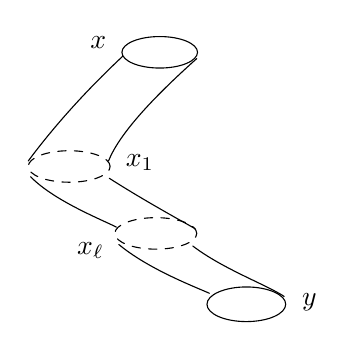
\begin{tikzpicture}[line cap=round,line join=round]
\draw (1.5,3.3) ellipse (0.48 and 0.20);
\draw[dashed] (0.35,1.85) ellipse (0.52 and 0.20);
\draw[dashed] (1.45,1.0) ellipse (0.52 and 0.20);
\draw (2.6,0.1) ellipse (0.5 and 0.22);
\draw (1.03,3.25) .. controls (0.55,2.8) and (0.15,2.35) .. (-0.17,1.92);
\draw (1.97,3.22) .. controls (1.5,2.8) and (1.0,2.3) .. (0.85,1.92);
\draw (-0.14,1.72) .. controls (0.15,1.42) and (0.75,1.18) .. (0.95,1.08);
\draw (0.86,1.7) .. controls (1.25,1.45) and (1.7,1.2) .. (1.95,1.06);
\draw (0.98,0.86) .. controls (1.35,0.55) and (1.95,0.32) .. (2.13,0.24);
\draw (1.92,0.84) .. controls (2.3,0.55) and (2.85,0.35) .. (3.08,0.2);
\node at (0.72,3.42) {$x$};
\node at (1.25,1.9) {$x_{1}$};
\node at (0.62,0.78) {$x_{\ell}$};
\node at (3.4,0.12) {$y$};
\end{tikzpicture}
\caption{}
\label{fig:broken-trajectory-tubes}
\end{figure}

\begin{proof}[\cref{thm:broken-limit-decomposition}的证明]
我们使用\cref{thm:trajectories-tend-critical-points}的证明中所用的记号。特别地，$\varepsilon$ 取得充分小，使得以 $\scr{A}_{H}$ 的诸\trCriticalPoint{}为中心、半径为 $\varepsilon$ 的各个球两两不相交。对 $u\in\scr{M}$，我们令 $u(s)\in\scr{L}W$ 表示\trLoop{} $u(s,t)$。

视为 $\scr{L}W$ 中的一条\trTrajectory，$u_{n}$ 必定要离开 $B(x,\varepsilon)$，因为它最终要到达 $y$。设 $u_{n}(s_{n}^{1})$ 是它的第一个\textbf{\trExitPoint}（exit point），
\[
s_{n}^{1}=\inf\bigl\{s\in\RR\mid d_{\infty}\bigl(u_{n}(s),x\bigr)>\varepsilon\bigr\}\text{。}
\]
由 $\scr{M}$ 的\trCompact{}性（并且在必要时抽取一个子序列之后），序列 $(u_{n}\cdot s_{n}^{1})$ \trConvergence{}到 $\scr{M}$ 的一个元素 $u^{1}$。按 $s_{n}^{1}$ 的定义，我们有
\[
\begin{cases}
d_{\infty}\bigl(u_{n}(s),x\bigr)<\varepsilon &\text{对 } s<s_{n}^{1}\text{，}\\[4pt]
d_{\infty}\bigl(u_{n}(s_{n}^{1}),x\bigr)=\varepsilon\text{，} &
\end{cases}
\]
从而在极限情形，
\[
u^{1}(s)\in\overline{B}(x,\varepsilon)\quad\text{对 } s<0\qquad\text{并且}\qquad u^{1}(0)\in\partial B(x,\varepsilon)\text{。}
\]
于是，极限 $u^{1}$ 是一条从 $x$ 出发而穿出球 $B(x,\varepsilon)$ 的\trTrajectory。因而它也落在某个 $\scr{M}(x,x_{1})$ 之中，其中 $x_{1}\in\operatorname{Crit}\scr{A}_{H}$（异于 $x$）。若 $x_{1}=y$，那么我们就大功告成（此时 $\ell=0$）。若不然，我们就使用归纳法：我们假定已经找到了诸序列 $(s_{n}^{0}),\dots,(s_{n}^{k})$ 与诸元素 $u^{j}\in\scr{M}(x_{j-1},x_{j})$（对应于 $\scr{A}_{H}$ 的某些\trCriticalPoint）\footnote{译注：原书\cref{thm:broken-limit-decomposition}以 $0$ 起标——诸元素 $u^{k}\in\scr{M}(x_{k},x_{k+1})$（$k=0$ 即 $u^{0}\in\scr{M}(x_{0},x_{1})$）、诸序列 $(s_{n}^{k})$（$0\le k\le\ell$）；而证明先构造的却是 $u^{1}$（对应第一\trExitPoint{} $s_{n}^{1}$，落在 $\scr{M}(x,x_{1})$ 之中），本句归纳假设又写 $(s_{n}^{0}),\dots,(s_{n}^{k})$ 与 $u^{j}\in\scr{M}(x_{j-1},x_{j})$——两套起标错开一位，且 $(s_{n}^{0})$ 于证明中从未定义。按证明的实际构造，诸序列应自 $(s_{n}^{1})$ 起统一作 $1$ 起标（或全部对齐定理的 $0$ 起标）。此处照原书排印，存疑备案。——译者注}，其中 $x_{j}\neq y$，并且
\[
\lim_{n\to\infty}u_{n}\cdot s_{n}^{j}=u^{j}\text{。}
\]
当 $s$ 趋于 $+\infty$ 时，\trTrajectory{} $u^{k}$ 趋于\trCriticalPoint{} $x_{k}$，于是存在一个 $s^{\star}\in\RR$，使得
\[
\forall s\ge s^{\star}\text{，}\quad u^{k}(s)\in B(x_{k},\varepsilon)\text{。}
\]

由于 $u_{n}\cdot s_{n}^{k}(s^{\star})$ 趋于 $u^{k}(s^{\star})$，故对充分大的 $n$，我们还有
\[
u_{n}(s_{n}^{k}+s^{\star})\in B(x_{k},\varepsilon)\text{。}
\]
由于\trTrajectory{} $(u_{n})$ 趋于 $y$——我们已假定它异于 $x_{k}$——它必定要在 $s>s_{n}^{k}+s^{\star}$ 时离开 $B(x_{k},\varepsilon)$。考虑第一个\trExitPoint{} $u_{n}(s_{n}^{k+1})$，其中
\[
s_{n}^{k+1}=\sup\bigl\{s\ge s_{n}^{k}+s^{\star}\mid u_{n}(\sigma)\in B(x_{k},\varepsilon)\ \text{对 } s_{n}^{k}+s^{\star}\le\sigma\le s\bigr\}\text{。}
\]
再由 $\scr{M}$ 的\trCompact{}性（并且在必要时抽取一个子序列之后），序列 $u_{n}\cdot s_{n}^{k+1}$ \trConvergence{}到一个极限 $u^{k+1}\in\scr{M}$。

\begin{figure}[htbp]
\centering
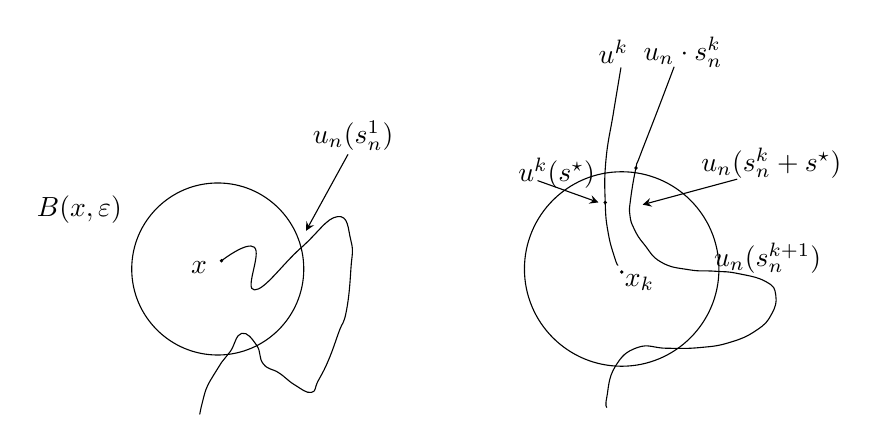
\begin{tikzpicture}[>=stealth,line cap=round,line join=round,scale=0.95]
\draw (0,0) circle (1.15);
\node at (-1.85,0.8) {$B(x,\varepsilon)$};
\fill (0.05,0.11) circle (0.025);
\node at (-0.25,0.02) {$x$};
\draw plot[smooth, tension=0.8] coordinates {(0.05,0.11) (0.49,0.29) (0.49,-0.28) (1.11,0.28) (1.60,0.70) (1.78,0.38) (1.78,0.0) (1.72,-0.56) (1.62,-0.84) (1.48,-1.22) (1.34,-1.50) (1.25,-1.65) (1.03,-1.55) (0.82,-1.39) (0.61,-1.27) (0.52,-1.02) (0.32,-0.86) (0.17,-1.10) (0.05,-1.25) (-0.05,-1.41) (-0.14,-1.57) (-0.19,-1.72) (-0.22,-1.84) (-0.24,-1.94)};
\node (un1) at (1.81,1.78) {$u_{n}(s_{n}^{1})$};
\draw[->] (1.74,1.53) -- (1.18,0.51);
\begin{scope}[xshift=5.4cm]
\draw (0,0) circle (1.3);
\fill (0,-0.04) circle (0.025);
\node at (0.24,-0.18) {$x_{k}$};
\draw plot[smooth, tension=0.8] coordinates {(-0.01,2.69) (-0.11,2.09) (-0.21,1.46) (-0.22,0.89) (-0.18,0.48) (-0.09,0.14) (-0.05,0.05)};
\fill (-0.22,0.89) circle (0.025);
\draw plot[smooth, tension=0.8] coordinates {(0.70,2.70) (0.48,2.12) (0.24,1.50) (0.19,1.35) (0.12,0.94) (0.11,0.72) (0.17,0.53) (0.30,0.33) (0.53,0.09) (0.90,-0.01) (1.25,-0.03) (1.55,-0.06) (1.93,-0.17) (2.06,-0.35) (2.00,-0.61) (1.80,-0.82) (1.45,-0.98) (1.05,-1.05) (0.61,-1.06) (0.21,-1.05) (-0.09,-1.31) (-0.20,-1.72) (-0.20,-1.85)};
\fill (0.19,1.35) circle (0.025);
\node at (-0.11,2.9) {$u^{k}$};
\node at (0.82,2.9) {$u_{n}\cdot s_{n}^{k}$};
\node at (-0.87,1.28) {$u^{k}(s^{\star})$};
\draw[->] (-1.12,1.18) -- (-0.31,0.89);
\node at (2.0,1.42) {$u_{n}(s_{n}^{k}+s^{\star})$};
\draw[->] (1.54,1.20) -- (0.28,0.86);
\node at (1.95,0.15) {$u_{n}(s_{n}^{k+1})$};
\end{scope}
\end{tikzpicture}
\caption{}
\label{fig:exit-points}
\end{figure}

我们现在要证明的是：所论的这条\trTrajectory{} $u^{k+1}$ 落在某个空间 $\scr{M}(x_{k},x_{k+1})$ 之中，其中 $x_{k+1}$ 是一个异于 $x_{k}$ 的\trCriticalPoint。我们先来验证 $s_{n}^{k+1}-s_{n}^{k}$ 趋于无穷。的确，假如相反地我们假定它是\trBounded{}的，那么区间 $[s^{\star},s_{n}^{k+1}-s_{n}^{k}]$ 就含于一个固定的紧区间……之中，在其上 $u_{n}\cdot s_{n}^{k}$ \trUniformConvergence{}到 $u^{k}$。从而，对 $s\in[s^{\star},s_{n}^{k+1}-s_{n}^{k}]$，我们有 $u_{n}(s_{n}^{k}+s)\in B(x_{k},\varepsilon)$，于是特别地，$u_{n}(s_{n}^{k+1})$ 就落在这个开球之中，这就引出了矛盾（因为按构造，$u_{n}(s_{n}^{k+1})\in\partial B(x_{k},\varepsilon)$）。因此 $s_{n}^{k+1}-s_{n}^{k}$ 的确趋于 $+\infty$。

设 $s$ 是一个负实数。对充分大的 $n$，我们有
\[
s_{n}^{k}+s^{\star}<s_{n}^{k+1}+s<s_{n}^{k+1}\text{，}
\]
于是按 $s_{n}^{k+1}$ 的定义，$u_{n}(s_{n}^{k+1}+s)\in B(x_{k},\varepsilon)$。从而对每个 $s<0$，我们都有\footnote{译注：原书此式左端未带求值记号，径印作 $u_{n}\cdot s_{n}^{k+1}\in B(x_{k},\varepsilon)$；按句首“对每个 $s<0$”的量词以及本页首行 $u_{n}\cdot s_{n}^{k}(s^{\star})$ 的求值写法，疑应在左端补出 $(s)$（即 $(u_{n}\cdot s_{n}^{k+1})(s)\in B(x_{k},\varepsilon)$，与前句等价；若把左端整体读作平移后的那条\trLoop，亦通）。此处照原书排印，存疑备案。——译者注}
\[
u_{n}\cdot s_{n}^{k+1}\in B(x_{k},\varepsilon)
\]
从而
\[
u^{k+1}\bigl(\,]-\infty,0]\bigr)\subset\overline{B}(x_{k},\varepsilon)\text{。}
\]
对 $s=0$，我们有 $u_{n}(s_{n}^{k+1})\in\partial B(x_{k},\varepsilon)$，故在极限下，
\[
u^{k+1}(0)\in\partial B(x_{k},\varepsilon)\text{，}
\]
于是 $u^{k+1}$ 必定要离开球 $B(x_{k},\varepsilon)$，而这正是我们所要证明的。
\end{proof}
